\section{刀具磨损预测神经网络}
% 
% 
\subsection{基于RNN的刀具磨损量预测模型}
\begin{frame}{基于循环神经网络刀具磨损量预测数学模型}
\ \ \ \ \ \ 我们试图寻找一种可以在机床工作时也可以测定刀具磨损度的预测方法,我们先对高维信号进行特征工程处理,在此基础上,将所获得的特征值与一维数据结合,运用循环神经网络模型对刀具磨损量进行预测。\par
% 
% 
\begin{figure}[htp]
    \centering
    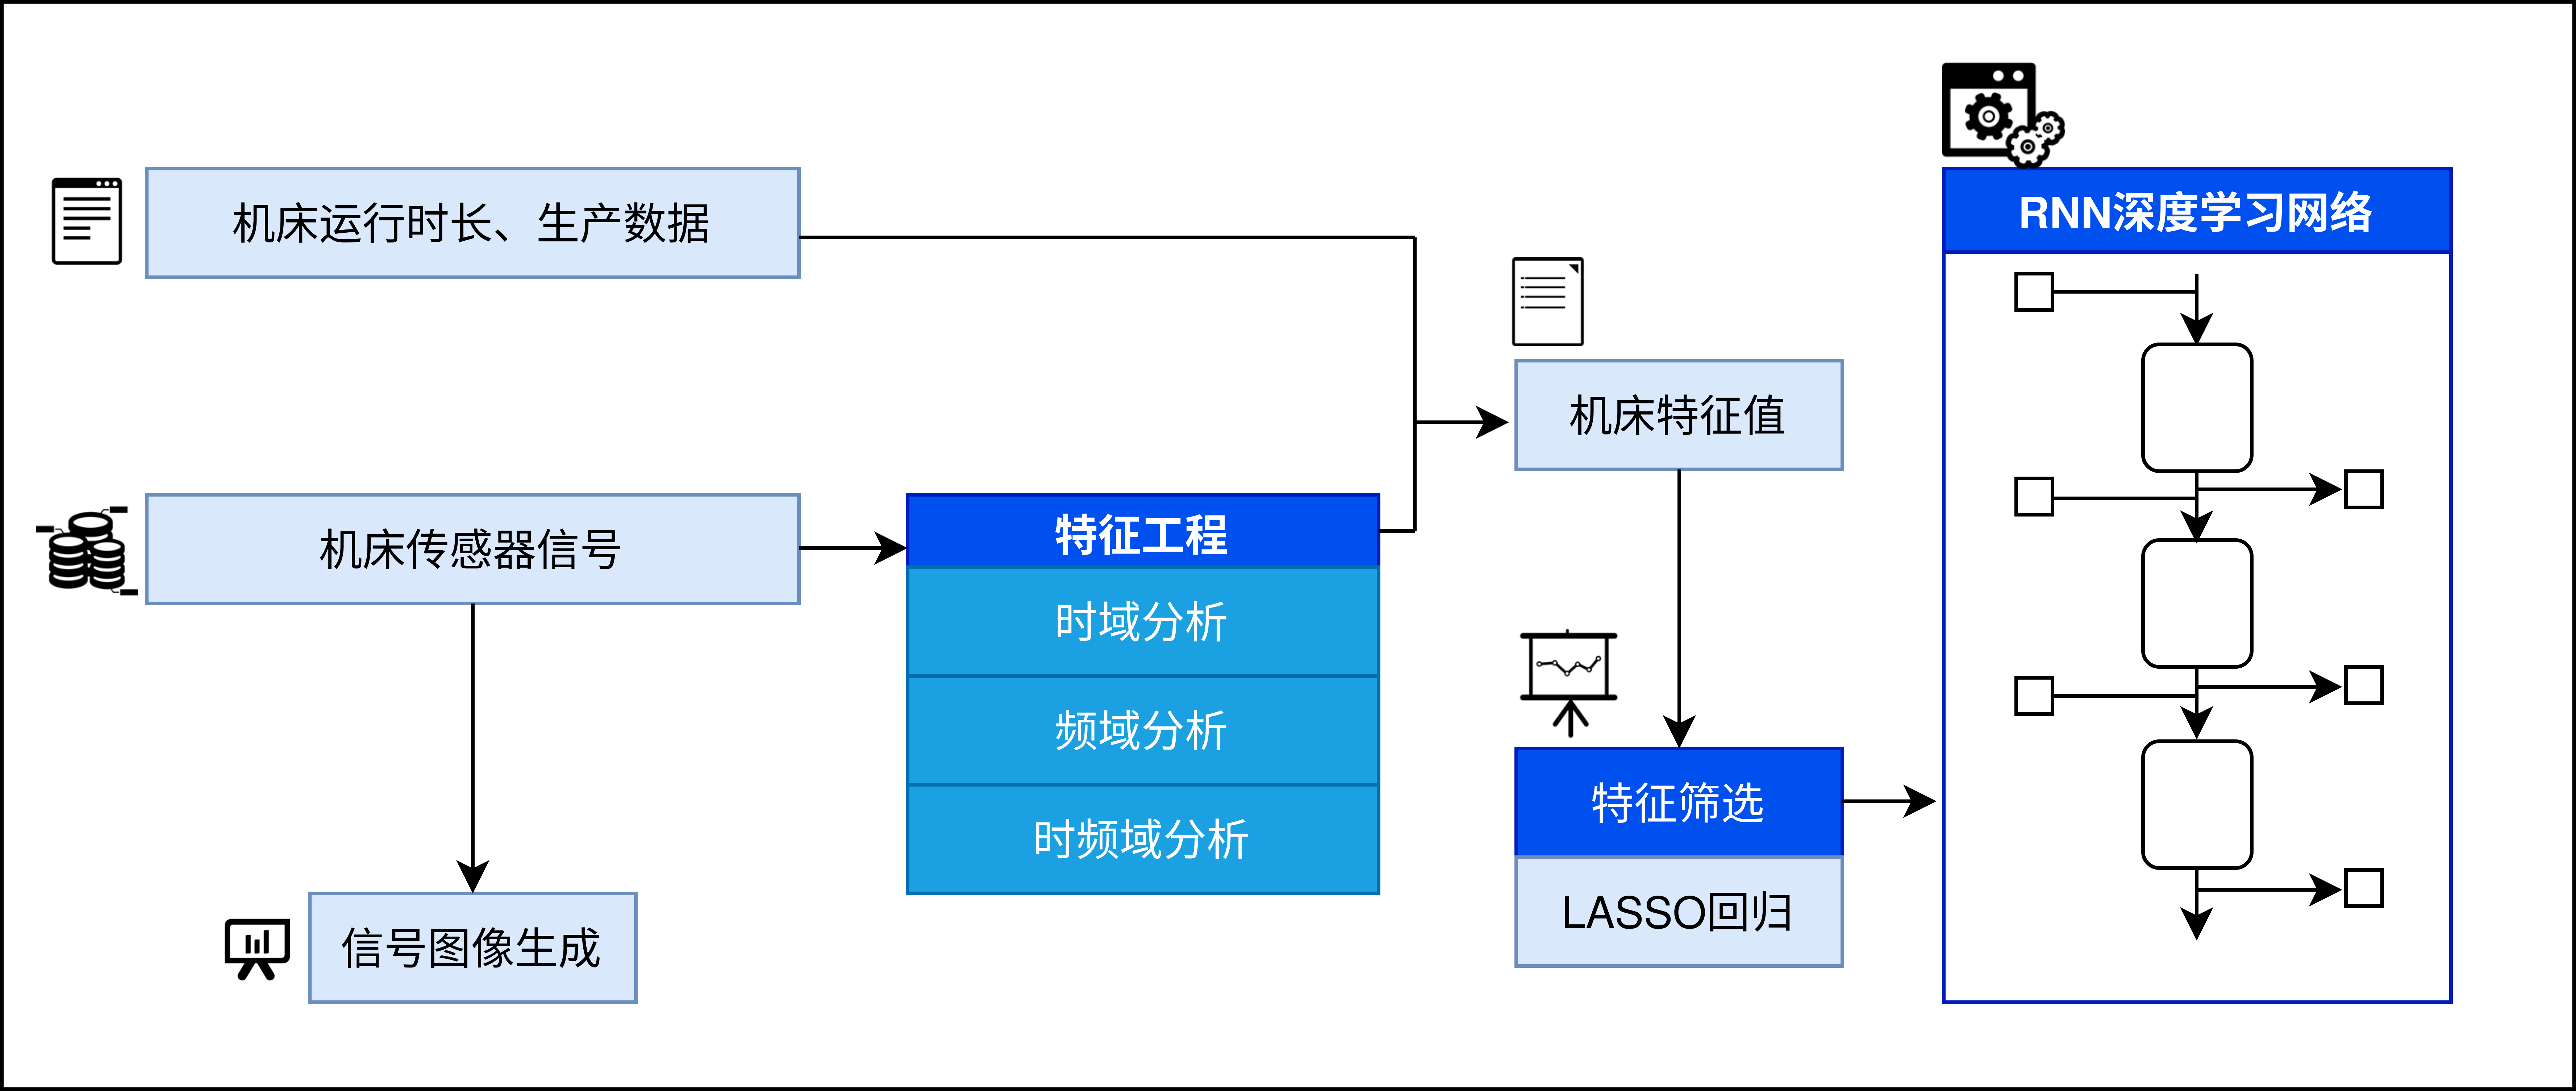
\includegraphics[width=12cm]{刀具磨损量预测神经网络/RNN测定模型.png}
    \caption{刀具磨损预测流程图}
\end{figure}
% 
% 
\end{frame} 
% 
% 
\begin{frame}{信号处理——时域特征提取}
\ \ \ \ \ \ 对于时域特征的提取,我们将有量纲特征值与无量纲特征值相结合,以时间为自变量表示目标信号数据的波形,具体特征如下:
\begin{minipage}[t]{0.45\textwidth}
\centering
$$ 绝对均值: |\bar{x}|=\frac{1}{N} \sum_{i=1}^{N}\left|x_{i}\right| $$\par
$$ 峭度值:x_{ra}=\left(\frac{1}{N} \sum_{i=1}^{N} \sqrt{|x_i|}\right)^{2} $$\par
$$ 均方根值:x_{rms}=\sqrt{\frac{1}{N} \sum_{k=1}^{N} x_{i}^{2}} $$\par
$$ 方根幅值:x_{kurtosis}=\frac{1}{N} \sum_{k=1}^{N}(x)^{n} $$\par
\end{minipage}
\begin{minipage}[t]{0.45\textwidth}
\centering
$$ 峰值:x_{pesk}=X_{max} $$\par
$$ 波形因子:f_{shape}=\frac{x_{rms}}{|\bar{x}|} $$\par
$$ 脉冲因子:f_{pulse}=\frac{x_{peak}}{|x|} $$\par
$$ 峰值因子:f_{crest}=\frac{x_{peak}}{x_{rms}} $$\par
$$ 裕度因子:f_{celearance}=\frac{x_{peak}}{x_{ra}} $$\par
\end{minipage}
\end{frame} 
% 
% 
\begin{frame}{信号处理——频域特征提取}
\ \ \ \ \ \ 但是只有时域特征的铣削力存在波动较大以及不同刀具差异较大的情况,因此,只有时域特征不够完善,需进一步建立频域和时频域的特征提取。\par
\ \ \ \ \ \ 我们采取频谱分析法提取铣刀切削原始信号的频域特征,具体特征如下:
\begin{minipage}[t]{0.45\textwidth}
\centering
$$ 重心频率:F_{FC}=\frac{\int_{0}^{+\infty}f(t)FFT(t)dt}{\int_{0}^{+\infty} FFT(t)dt} $$\par

\end{minipage}
\begin{minipage}[t]{0.45\textwidth}
\centering
$$ 均方频率:F_{MSF}=\frac{\int_{0}^{+\infty} FFT(t)f(t)^{2}dt}{\int_{0}^{+\infty}FFT(t)dt} $$\par
\end{minipage}
$$ 均方根频率:F_{RMSF}=\sqrt{\frac{\int_{0}^{+\infty}FFT(t)f(t)^{2}dt}{\int_{0}^{+\infty}FFT(t)dt}} $$ \par
$$ 频率方差: F_{VF}=\frac{\int_{0}^{+\infty}(f(t)-\frac{\int_{0}^{+\infty}f(t)FFT(t)dt}{\int_{0}^{+\infty}FFT(t)dt} )^{2}dt}{\int_{0}^{+\infty}FFT(t)dt}  $$ \par
\end{frame}
% 
% 
\begin{frame}{Matlab信号处理}
\begin{figure}[htbp]
% \centering
\begin{minipage}[t]{0.48\textwidth}
\centering
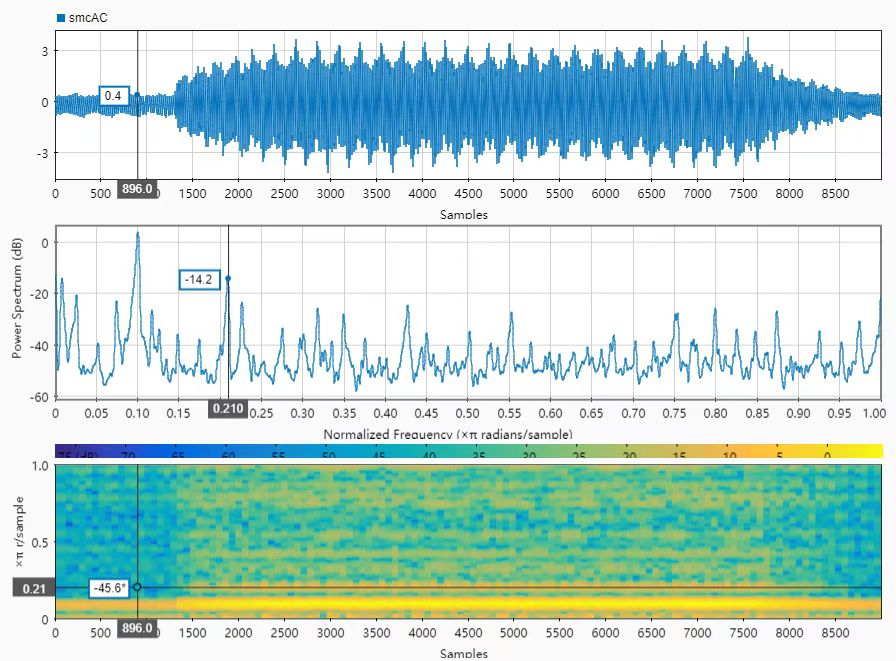
\includegraphics[width=6cm]{刀具磨损量预测神经网络/smcAC.jpg}
% \label{fig_22}
\caption{信号处理:smcAC}
\end{minipage}
\begin{minipage}[t]{0.48\textwidth}
\centering
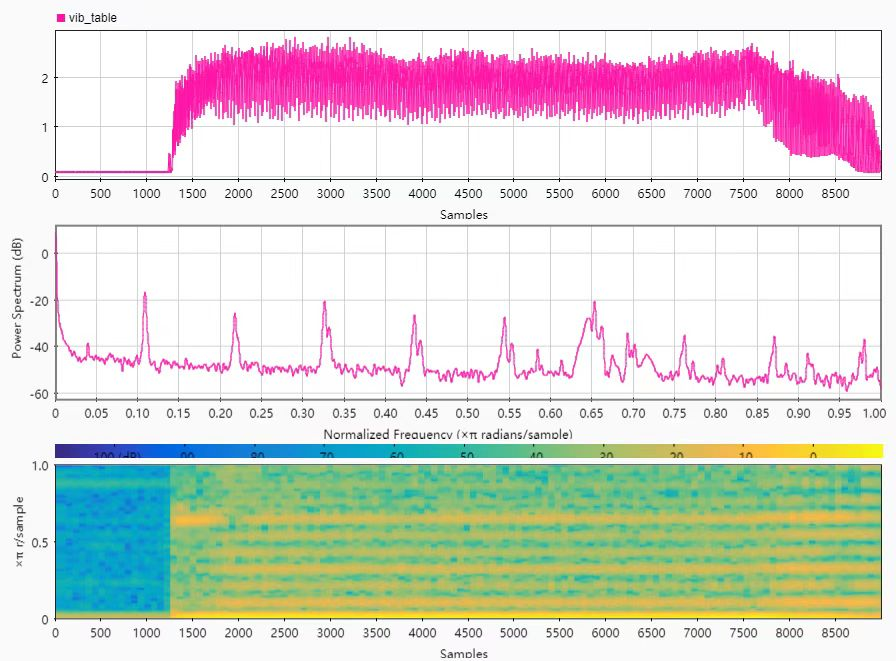
\includegraphics[width=6cm]{刀具磨损量预测神经网络/vib_table.jpg}
  \caption{信号处理:vib\_table}
% \label{fig_23}
\end{minipage}
\end{figure}
\end{frame}
% 
% 
% \subsubsection{特征筛选}
\begin{frame}{特征筛选——LASSO回归}
\ \ \ \ \ \ 每一次的铣削过程都对应着数万条信号数据和一个真实的铣刀磨损值,但并非所有采集到的信号数据都与刀具磨损量有着相关的关系,且经过各式传感器采集得到的原始信号的数据量过于庞大,原始信号数据当中还夹杂存在着各种干扰噪声,将其直接应用于刀具磨损量分析预测会大大增大方法实现的难度。因而需要通过进行合理适当的特征工程,在海量原始信号数据当中筛选出对研究目标对象刀具磨损量较为敏感的特征。\par
% F-test检验方法的原理是:假设特征矩阵为X,目标值为y,特征序号为i,使用函数mean()、std()和size()来分别表示计算特征矩阵平均值、特征矩阵标准差和目标长度,均值中心化则使用centered来表示。\par
% \ \ \ \ \ \ 因此相关系数Corr的公式为:\par
% $$ Corr=\frac{(X[:, i]-mean(X[:, i]))^{*}(y-mean(y))}{std(X[:, i])^{*} std(y)} $$ \par
% % 
% \ \ \ \ \ \ 自由度n的公式为:\par
% $$ n=size(y)-\left\{\begin{array}{l}
% 2\ \ \ if\ X,\ y\ centered \\
% 1\ \ \ if\ X,\ y\ not\ centered 
% \end{array}\right. $$ \par
% % 
% \ \ \ \ \ \ 基于此可以评估检验特征矩阵与目标值之间具有的线性关系,F-test评估检验值大于0.5的标准来进行特征选择。通过建立上述特征选择分析论证得出在各通道信号中声发射信号并没有贡献出与刀具磨损量相关的最优特征,因此在本研究的实验阶段将舍弃声发射信号通道的数据。\par
\ \ \ \ \ \ LASSO方法压缩回归模型的系数,其通过下式估计模型中的参数: \par
$$ \hat{\beta}_{Lasso}=\underset{\beta \in R^d}{arg\min}\left\{ \left. \sum_{i=1}^n{\left( y_i-\beta _ix_i \right) ^2+\lambda \sum_{j=1}^p{\left| \beta _j \right|}} \right\} \right.  $$
具体算法步骤如下:\par
\ \ \ \ \ \ (1)初始化$\delta _0 = sign\left( \beta ^0 \right)$,$\beta ^0$是最小二乘估计值。\par
\ \ \ \ \ \ (2)寻找$\hat{\beta}^{0}$,k表示第k次寻找,使得误差平方和$J\left( \beta \right)=\sum_{i=1}^{i=n}{\left( y_i-\sum_{j=1}^p{\beta _jx_{ij}^2} \right)}$达到最小。\par
% $$ J\left( \beta \right) =\sum_{i=1}^{i=n}{\left( y_i-\sum_{j=1}^p{\beta _jx_{ij}^2} \right)} $$\par
\ \ \ \ \ \ (3)$\delta _0=sign\left( \beta ^0 \right) $,当$\delta _{k}^{T}\hat{\beta}^k \le t$,$\hat{\beta}^{0}$即为Lasso回归方法的最优解;否则返回步骤(2)继续寻找。\par
% 
\ \ \ \ \ \ 通过建立特征选择分析论证得出在各通道信号中某些信号并没有贡献出与刀具磨损量相关的最优特征,因此在本研究的实验阶段将舍弃那些信号通道的特征值。 \par
\end{frame}

\begin{frame}{基于RNN的加工中心刀具退化预测}
\ \ \ \ \ \ 输入层:当前加工人物数据及筛选后的信号特征值$X_{t} \in R^{n*d}$ \\
\ \ \ \ \ \ 隐藏状态层:前置加工隐藏状态矩阵$H_{t-1} \in R^{n*h} $ \\
\ \ \ \ \ \ 输出层:刀具退化预测值$O_t \in R^{n*1}$
\begin{figure}[htp]
    \centering
    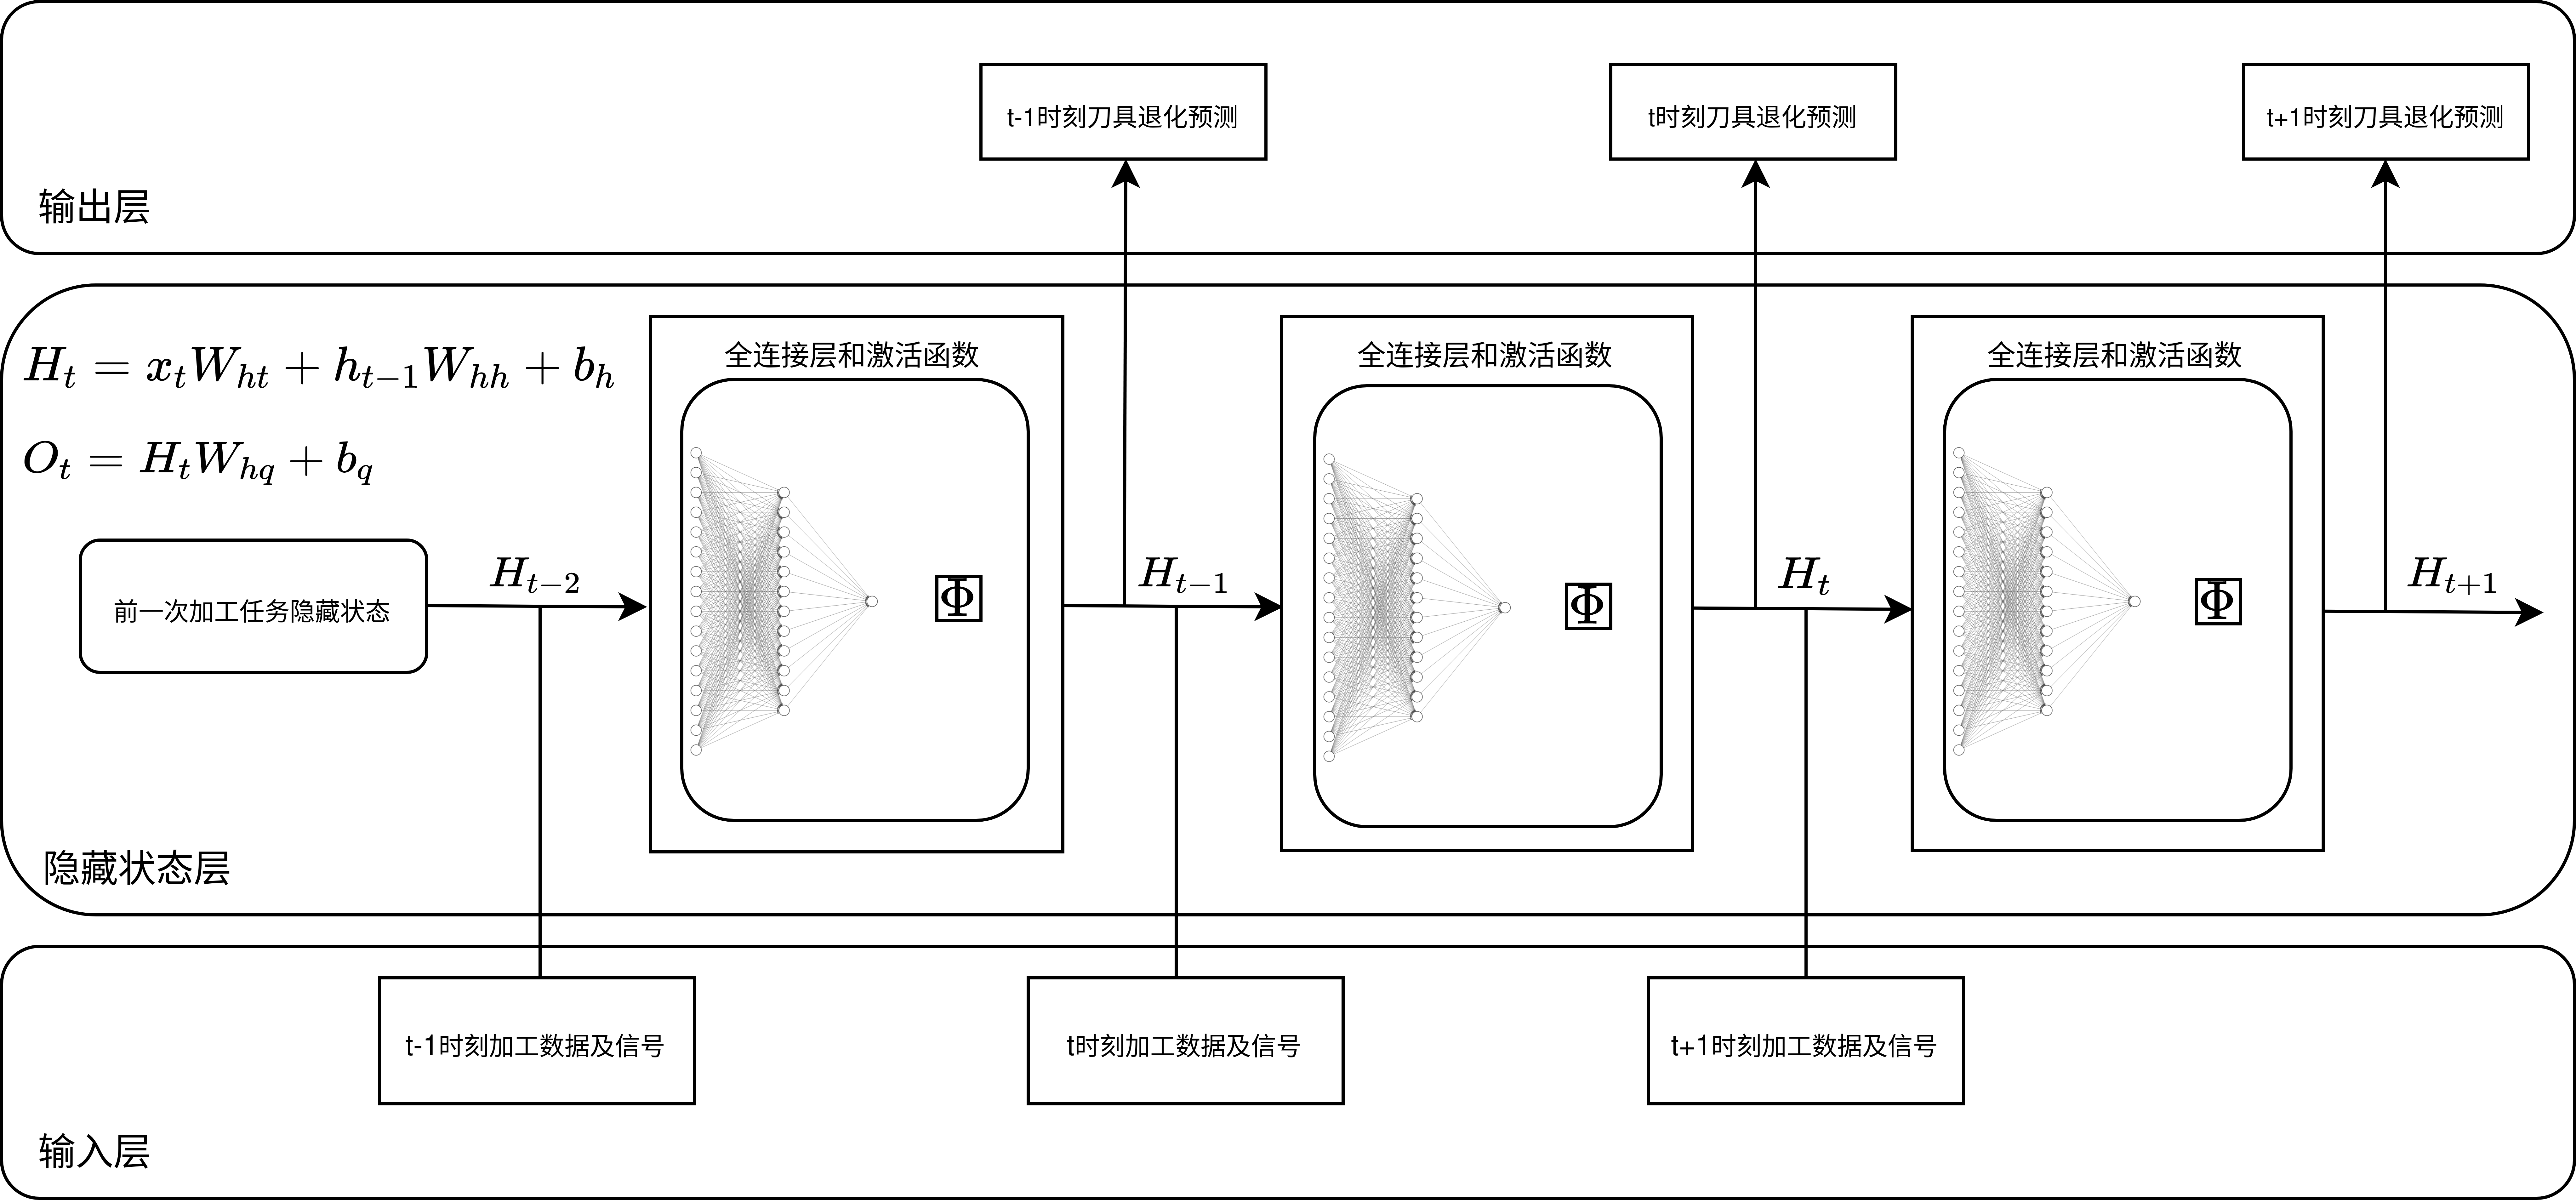
\includegraphics[width=10cm]{刀具磨损量预测神经网络/RNN architecture.png}
    \caption{循环神经网络架构}
\end{figure}
\end{frame}
% 
% 
% 
% 
% 
% 
% 
% 